\begin{enumerate}
	\item The pair of linear equations $ 2x=5y+6 $ and $ 15y=6x-18 $ represents two lines which are : 
\begin{enumerate}
    \item intersecting
    \item parallel
    \item coincident
    \item either intersecting or parallel
\end{enumerate}
\item Two schools $P$ and $Q$ decided to award prizes to their students for two games of Hockey \rupee $x$ per students and cricket \rupee $y$ per student. School $P$
decided to award a total of \rupee $9,500$ for the two games to $5$ and $4$ students respectively; while school $Q$ decided to award \rupee $7,370$ for the two games to $4$ and $3$ students respectively.
\begin{figure}[H]
    \centering
    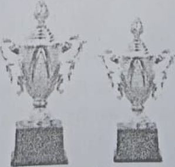
\includegraphics[width=\columnwidth]{figs/math.png}
    \caption{trophies}
    \label{fig:trophies}
\end{figure}


Based on the given information, answer the following questions :
\begin{enumerate}[label=(\roman*)]
    \item Represent the following information algebraically(in terms of $x$ and $y$).
    \item\begin{enumerate}[label=(\alph*)]
\item what is the prize amount for hockey ?
\item Prize amount on which game is more and by how much ?
    \end{enumerate}
    \item what will be the total prize amount if there are $2$ students each from two games ?
\end{enumerate}
\item If the pair of equations $3x - y + 8 = 0$ and $6x - ry +16 =0$ represents coincident lines,then the values of $r$ is :
\begin{enumerate}[label=(\alph*)]
    \item $-\frac{1}{2}$
    \item $\frac{1}{2}$
    \item $2$
    \item $-2$
\end{enumerate}
\item The pair of equations $x=a$ and $y=b$ graphically represents lines which are :
\begin{enumerate}[label=(\alph*)]
    \item parallel
    \item intersecting at $\brak{b,a}$
    \item coincident
    \item intersecting at $\brak{a,b}$
\end{enumerate}
\item
\begin{enumerate}[label=(\alph*)]
\item If the system of linear equations 
$2x + 3y = 7$  and   $2ax +\brak{a + b}y =28$ 
have infinite number of solutions, then find the values of $a$ and $b$.
\item  If $217x + 131y = 913$ and  
$131x + 217y = 827$,  then solve the equations for the values of $x$ and $y$.
\end{enumerate}
\item Half of the difference between two numbers is $2$. The sum of the greater number and twice the smaller number is $3$.Find the numbers.
\end{enumerate}
